\section{Aufbau}
\label{sec:Aufbau}
In diesem Versuch wird ein Sagnac-Interferometer verwendet. Dieses ist in \autoref{fig:Sagnac}
schematisch dargestellt. 
Das Interferometer besteht aus einem HeNe-Laser, der linear polarisiertes Licht der Wellenlänge $632.99\,\unit{\nano\meter}$
emittiert, und aus mehreren Spiegeln. Das Licht des Lasers ist in dessen Polarisation außerdem um 45° gegenüber der Vertikalen gekippt.
Die ersten beiden Spiegel M1 und M2 dienen dazu, den Laser in das Interferometer zu lenken. Die weiteren drei Spiegel $\symup{M_A}$, 
$\symup{M_B}$ und $\symup{M_C}$ sind Teil des Interferometers. Des Weiteren enthält es ein PBSC, der den Laserstrahl teilt.
Zur Justage liegen dem Versuch 2 Justageplatten sowie Metallplättchen bei. Außerdem stehen ein Schirm, ein 45°-Polarisationsfilter und ein um 45°-gedrehter
PBSC zur Verfügung. Die polarisierten Strahlen werden dann in zwei verschiedene PFotodioden gelenkt.
Die Messung erfolgt mit Hilfe der sogenannten Differenzspannungsmethode.
Bei Anwendung dieser Methode liegt der Vorteil darin, 
dass hinterher die beiden Signale voneinander abgezogen werden und somit äußere Störfaktoren wie Restlicht im Laborraum systematisch herausgerechnet werden können.
Unter anderem durch diese Methode ist das Sagnac-Interferometer nicht so störungsempfindlich wie andere Interferometer.
Für die Messung enthält der Versuch zwei verkippte dünne Glasplatten mit der Dicke $T=1\,\mathrm{mm}$, eine Gaszelle, Photodioden sowie
ein Oszilloskop.
\begin{figure}
    \centering
    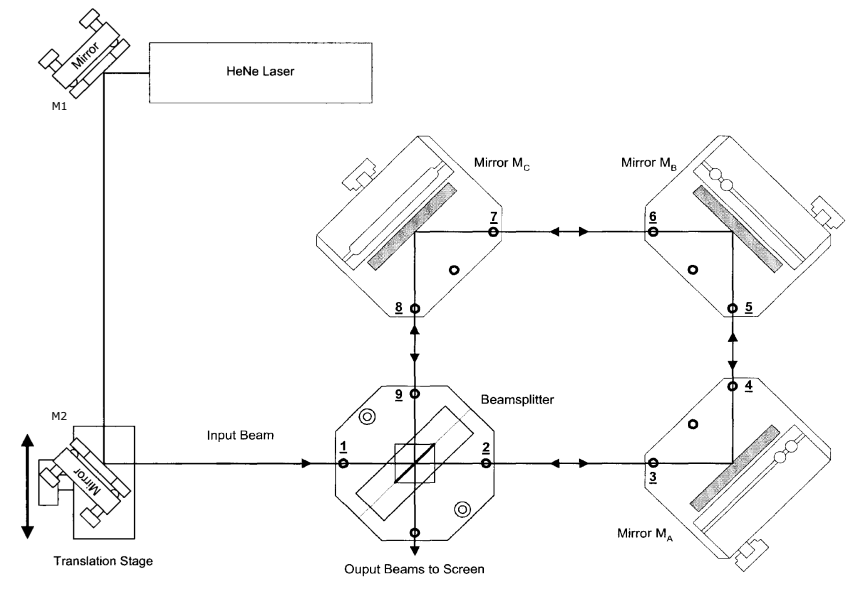
\includegraphics[width=0.8\textwidth]{Sagnac.png}
    \caption{Schematischer Aufbau eines Sagnac-Interferometers \cite{ap64}.}
    \label{fig:Sagnac}
\end{figure}